\chapter[Declaration on Scientific Integrity]{Declaration on Scientific Integrity\\Erklärung zur wissenschaftlichen Redlichkeit}
\label{DeclarationOfAuthorship}

includes Declaration on Plagiarism and Fraud \\
beinhaltet Erklärung zu Plagiat und Betrug \vspace{1cm}

\formlabel{Author}{Autor}
\authorsint

\formlabel{Matriculation number}{Matrikelnummer}
\immatriculnrint

\formlabel{Title of work}{Titel der Arbeit}
\titleint

\formlabel{Type of work}{Typ der Arbeit}
\thesistypeint

\formlabel{Declaration}{Erklärung}
I hereby declare that this submission is my own work and that I have fully acknowledged the assistance received in completing this work and that it contains no material that has not been formally acknowledged. 
I have mentioned all source materials used and have cited these in accordance with recognised scientific rules.

\vspace{0.3cm}

Hiermit erkläre ich, dass mir bei der Abfassung dieser Arbeit nur die darin angegebene 
Hilfe zuteil wurde und dass ich sie nur mit den in der Arbeit angegebenen Hilfsmitteln 
verfasst habe. Ich habe sämtliche verwendeten Quellen erwähnt und gemäss anerkannten wissenschaftlichen Regeln zitiert. 


\vspace*{0.5cm}

Basel, Oktober 12, 2020
\vspace*{0.25cm}

\begin{flushright}
\begin{figure}
    \raggedleft
    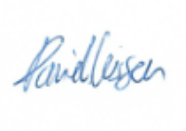
\includegraphics[]{UNTERSCHRIFT.PNG}
\end{figure}
\rule{75mm}{0.4pt} \\
\formlabel{Signature}{Unterschrift}
\end{flushright}
